\section{Background and Related Work} \label{sec:background}

In this chapter we explain the related work: we give a short overview 
about existing approaches and relevant methods. 

First, we describe the concept of a namespace from the Computer Science point
of view in section~\ref{sec:namespaces-cs}. Then we discuss how identifier 
definitions can be extracted, and for that we first introduce Part-of-Speech 
Tagging and its application to mathematical texts in section~\ref{sec:postagging},
and then review the extraction methods in section~\ref{sec:definition-extraction-methods}.

Next, section~\ref{sec:vsm}  describes the Vector Space Model, a traditional
way of representing a collection of documents as vectors, and then 
section~\ref{sec:similarity-distance} reviews common similarity and distance 
functions that are useful for document clustering. 

Finally, document clustering techniques are described in section~\ref{sec:doc-clustering},
and the Latent Semantic Analysis method for revealing semantic information from the 
document corpus is in section~\ref{sec:lsa}.


\subsection{Namespaces in Computer Science} \label{sec:namespaces-cs}

In computer science, a \emph{namespace} refers to a collection of terms
that are grouped because they share functionality or purpose,
typically for providing modularity
and resolving name conflicts \cite{duval2002metadata}.


\textbf{Example 1.} Namespaces are used in XML (eXtensible Markup Language), which
is a framework for defining markup languages \cite{moller2006introduction}.
However, different XML languages may use the same names for elements and attributes.
For example, consider two XML languages: XHTML for specifying the layout of web
pages, and some XML language for describing furniture. Both these languages have
the \verb|<table>| elements there, in XHTML table is used to present some data in
a tabular form, while the second one uses it to describe a particular piece of
furniture in the database.

The \verb|<table>| elements have very different semantics in these languages
and there should be a way to distinguish between these two elements.
In XML this problem is solved with XML namespaces~\cite{xmlnamespaces}:
the namespaces are used to ensure the uniqueness of attributes and resolve ambiguity.
It is done by binding a short namespace alias with some uniquely defined URI
(Unified Resource Identifier), and then appending the alias to
all attribute names that come from this namespace. In the example above,
we can bind an alias \verb|h| with XHTML's URI \url{http://www.w3.org/TR/xhtml1}
and then use \verb|<h:table>| to refer to XHTML's table. Likewise,
in the furniture database language the element names can be prepended
with a prefix \verb|d|, where \verb|d| is bound to some URI, e.g.
\url{http://www.furniture.de/2015/db}.


% Ralf's comment: ``namespaces" were deeply studied mainly in
% the field of distributed systems/ middleware (like DCE, CORBA, etc.) in the middle
% of the 80s/ 90s ...


\textbf{Example 2.} Namespaces are also used in programming languages for organizing
variables, procedures and other identifiers into groups and
for resolving name collisions. In programming languages without
namespaces the programmers have to take special care to avoid
naming conflicts. For example, in the PHP programming language
prior to version 5.3 \cite{mcarthur2008php6} there is no notion of namespace, and
the namespaces have to be emulated to ensure that the names
are unique, and 
\verb|Zend_Search_Lucene_Analysis_Analyzer|\footnote{\url{http://framework.zend.com/apidoc/1.7/Zend_Search_Lucene/Analysis/Zend_Search_Lucene_Analysis_Analyzer.html}}
and other long names is the result.

Other programming languages have the notion of namespaces built in
from the very first versions. For example, the Java programming
language~\cite{gosling2014java} uses packages to organize identifiers into
namespaces, and packages solve the problem of ambiguity. For example,
in the standard Java API there are two classes with the name \texttt{Date}:
one in the package \texttt{java.util} and another in the package \texttt{java.sql}.
To be able to distinguish between them, the classes are referred by their
\emph{fully qualified name}: an unambiguous name that uniquely specifies the class
by combining the package name with the class name. Thus, to refer to a particular
\texttt{Date} class in Java  \texttt{java.util.Date} or  \texttt{java.sql.Date}
should be used.

It is not always convenient to use the fully qualified name in the code to
refer to some class from another package. Therefore in Java it is possible to
\emph{import} the class by using the import statement which associates
a short name alias with its fully qualified name.
For example, to refer to \texttt{java.sql.Date} it is possible to import
it by using \texttt{import java.sql.Date} and then refer to it by the alias
\texttt{Date} in the class \cite{gosling2014java}.


Although there are no strict rules about how to organize the classes into
packages, it is a good software design practice to put
related objects into the same namespace and by doing this achieve
better modularity. There are design principles that tell software engineers
how to best organize the source code: classes in a well designed system
should be grouped in such a way that namespaces
exhibit low \emph{coupling} and high \emph{cohesion}~\cite{larman2005applying}.
Coupling describes the degree of dependence between namespaces, and
low coupling means that the interaction between classes of different
namespaces should be as low as possible. Cohesion, on the other hand,
refers to the dependence within the classes of the same namespace,
and the high cohesion principle says that the related classes
should all be put together in the same namespace.


\subsection{Math-aware POS tagging} \label{sec:postagging}
Part-of-Speech Tagging (POS Tagging) is a typical Natural Language Processing
task which assigns a POS Tag to each word in a given text \cite{jurafsky2000speech}.
While the POS Tagging task is mainly a tool for text processing, it can
also be applicable to scientific documents with mathematical expressions,
and can be adjusted to dealing with formulae \cite{schoneberg2014pos}
\cite{pagael2014mlp}.

A \emph{POS tag} is an abbreviation that corresponds to some
part of speech. Penn Treebank POS Scheme \cite{santorini1990part} is
a commonly used POS tagging scheme which defines a set of part-of-speech tags
for annotating English words.
For example, \texttt{JJ} is an adjective (``big''), \texttt{RB} as in adverb,
\texttt{DT} is a determiner (``a'', ``the''), \texttt{NN} is a
noun (``corpus'') and \texttt{SYM} is used for symbols (``$>$'', ``$=$'').


However the Penn Treebank scheme does not have special tags for mathematics,
but it is flexible enough and can be extended to include additional tags.
For example, we can include a math-related tag \texttt{MATH}.
Usually it is done by first applying traditional POS taggers (like Stanford
CoreNLP \cite{manning2014stanford}), and then
refining the results by re-tagging math-related tokens of text as \texttt{MATH}
\cite{schoneberg2014pos}.


For example, consider the following sentence:
``The relation between energy and mass is
described by  the mass-energy equivalence formula $E = mc^2$,
where $E$ is energy, $m$ is mass and $c$ is the speed of light''.
In this case we will assign the \verb|MATH| tag to ``$E = mc^2$'', ``$E$'',
``$m$'' and ``$c$''

However we can note that for finding identifier-definition relations
the \texttt{MATH} tag alone is not sufficient: we need to distinguish
between complex mathematical expressions and stand-alone identifiers -
mathematical expressions that contain only one symbol: the identifier.
For the example above we would like to be able to distinguish the
expression ``$E = mc^2$'' from identifier tokens ``$E$'',
``$m$'' and ``$c$''. Thus we extend the Penn Treebank scheme even more
and introduce an additional tag \texttt{ID} to denote stand-alone identifiers.


Thus, in the example above ``$E = mc^2$'' will be assigned the \texttt{MATH} tag
and ``$E$'', ``$m$'' and ``$c$'' will be annotated with \texttt{ID}.

In the next section we discuss how this can be used to find identifier-definition
relations.


\subsection{Mathematical Definition Extraction} \label{sec:definition-extraction-methods}

In Natural Language Processing, Word Sense Disambiguation is a problem of
identifying in which sense a polysemous word is used \cite{jurafsky2000speech}.
Analogously, the Identifier Disambiguation problem is a problem of
determining the meaning of an identifier in a mathematical formula. This
problem is typically solved by extracting definitions from the natural
language description that surrounds the formula.

For example, given the sentence ``The relation between energy and mass is
described by  the mass-energy equivalence formula $E = mc^2$,
where $E$ is energy, $m$ is mass and $c$ is the speed of
light''\footnote{\url{https://en.wikipedia.org/wiki/Mass\%E2\%80\%93energy\_equivalence}}
the goal is to extract the following identifier-definition relations:
($E$, ``energy''), ($m$, ``mass'') and ($c$, ``the speed of light'').

Formally, a phrase that defines a mathematical expression consists of three parts \cite{kristianto2012extracting}:

\begin{itemize}
\itemsep1pt\parskip0pt\parsep0pt
  \item \emph{definiendum} is the term to be defined: it is a mathematical expression
      or an identifier;
  \item \emph{definiens} is the definition itself: it is the word or phrase that defines the definiendum in a definition;
  \item \emph{definitor} is a relator verb that links definiendum and definiens.
\end{itemize}

In this work, we are interested in the first two parts: \emph{definiendum} and
\emph{definiens}. Thus we define a \emph{relation} as a pair
(definiendum, definiens). For example, ($E$, ``energy'') is a relation where
``$E$'' is a definiendum, and ``energy'' is a definiens. We refer to definiendum as
identifier, and to definiens as definition, so relations are identifier-definition
pairs.

There are several ways of extracting the identifier-definition relations.
Here we will review the following:

\begin{itemize}
\itemsep1pt\parskip0pt\parsep0pt
  \item Nearest Noun
  \item Pattern Matching
  \item Machine-Learning based methods
  \item Probabilistic methods
\end{itemize}


\subsubsection{Nearest Noun Method} \ \\

The Nearest Noun  \cite{grigore2009towards} \cite{yokoi2011contextual}
is the simplest definition extraction method.
It assumes that the definition is a combination of ad
It finds definitions by looking for combinations of adjectives and nouns
(sometimes preceded by determiners) in the text before the identifier.

I.e. if we see a token annotated with \texttt{ID}, and then a sequence
consisting only of adjectives (\texttt{JJ}), nouns (\texttt{NN}, \texttt{NNS})
and determiners (\texttt{DET}), then we say that this sequence is
the definition for the identifer.

For example, given the sentence ``In other words, the bijection $\sigma$ normalizes
$G$ in ...'' we will extract a relation ($\sigma$, "bijection").



\subsubsection{Pattern Matching Methods} \label{sec:pattern-matching} \ \\

The Pattern Matching method \cite{quoc2010mining} is an extension of the
Nearest Noun method: In Nearest Noun, we are looking for one specific patten
where identifier is followed by the definition, but we can define several such
patterns and use them to extract definitions.

For example, we can define the following patterns:

\begin{itemize}
\itemsep1pt\parskip0pt\parsep0pt
  \item \texttt{IDE} \texttt{DEF}
  \item \texttt{DEF} \texttt{IDE}
  \item let$|$set \texttt{IDE} denote$|$denotes$|$be \texttt{DEF}
  \item \texttt{DEF} is$|$are denoted$|$\texttt{def}ined$|$given as$|$by \texttt{IDE}
  \item \texttt{IDE} denotes$|$denote$|$stand$|$stands as$|$by \texttt{DEF}
  \item \texttt{IDE} is$|$are \texttt{DEF}
  \item \texttt{DEF} is$|$are \texttt{IDE}
  \item and many others
\end{itemize}


In this method \texttt{IDE} and \texttt{DEF} are placeholders that are
assigned a value when the pattern is matched against some subsequence
of tokens.  \texttt{IDE} and DEF need to
satisfy certain criteria in order to be successfully matched: like in the
Nearest Noun method we assume that \texttt{IDE} is some token annotated with
\texttt{ID} and \texttt{DEF} is a phrase containing adjective (\texttt{JJ}),
nouns (\texttt{NN}) and  determiners (\texttt{DET}). Note that the first patten corresponds
to the Nearest Noun pattern.

The patterns above are combined from two lists: one is extracted from a
guide to writing mathematical papers in English (\cite{trzeciak1995writing}),
and another is extracted from ``Graphs and Combinatorics'' papers from Springer
\cite{kristianto2012extracting}.

The pattern matching method is often used as the baseline method
for identifier-definition extraction methods \cite{kristianto2012extracting}
\cite{kristianto2014extracting} \cite{pagael2014mlp}.


\subsubsection{Machine Learning Based Methods}

\ \\

The definition extraction problem can be formulated as a binary classification
problem: given a pair (identifier, candidate-definition), does this pair
correspond to a real identifier-definition relation?

To do this we find all candidate pairs: identifiers are tokens
annotated with \texttt{ID}, and candidate defections are nouns and
noun phrases from the same sentence as the definition.

Once the candidate pairs are found, we extract the following features
\cite{yokoi2011contextual} \cite{kristianto2014extracting}:


\begin{itemize}
\itemsep1pt\parskip0pt\parsep0pt
  \item boolean features for each of the patterns from
    section~\ref{sec:pattern-matching} indicating if the pattern is matched,
  \item indicator if there's a colon or comma between candidate and identifier,
  \item indicator if there's another math expression between candidate and identifier,
  \item indicator if candidate is inside parentheses and identifier is outside,
  \item distance (in words) between the identifier and the candidate,
  \item the position of candidate relative to identifier,
  \item text and POS tag of one/two/three preceding and following tokens around the candidate,
  \item text of the first verb between candidate and identifier,
  \item many others.
\end{itemize}

Once the features are extracted, a binary classifier can be trained to predict
if an unseen candidate pair is a relation or not.
For this task the popular choices of classifiers are Support Vector Machine
classifier with linear kernel \cite{kristianto2014extracting} \cite{yokoi2011contextual}
and Conditional Random Fields \cite{kristianto2014extracting},
but, in principle, any other binary classifier can be applied
as well.


\subsubsection{Probabilistic Approaches} \label{sec:mlp} \ \\

In the Mathematical Language Processing approach \cite{pagael2014mlp}
a definition for an identifier is extracted by ranking
candidate definitions by the probability of definining
the identifier, and only the most probable candidates are retained.

The main idea of this approach is that the definitions occur very closely
to identifiers in sentences, and the closeness can be used to
model the probability distribution over candidate definitions.

The candidates are ranked by the following formula:
$$R(n, \Delta, t, d) = \cfrac{\alpha \, R_{\sigma_d}(\Delta) + \beta \, R_{\sigma_s}(n) + \gamma \, \text{tf}(t)}{\alpha + \beta + \gamma}$$
where $\Delta$ is the number of tokens between the identifier and the definition
candidate, and $R_{\sigma_d}(\Delta)$ is a Gaussian that models this distance, parametrized
with $\sigma_d$; $n$ is the number of sentences between the definition candidate
and the sentence where the identifier occurs for the first time, and is a Gaussian
parameterized with $\sigma_s$; finally $\text{tf}(t)$ is a frequency of term $t$
in a sentence. All these quantities are combined together and $\alpha, \beta, \gamma$ are weighting parameters.

The following weighting parameters $\alpha, \beta, \gamma$ are proposed in
\cite{pagael2014mlp}: $\alpha = \beta = 1$ and $\gamma = 0.1$.



\subsection{Vector Space Model} \label{sec:vsm}

Vector Space Model is a statistical model for representing documents
in some vector space. It is an Information Retrieval
model \cite{manning2008introduction}, but it is also used for various
Text Mining tasks such as Document Classification \cite{sebastiani2002machine}
and Document Clustering \cite{oikonomakou2005review} \cite{aggarwal2012survey}.

In Vector Space Model we make two assumptions about the data:
(1) \emph{Bag of Words assumption}: the order of words is not important,
only word counts;
(2) \emph{Independence assumption}: we treat all words as independent.
Both assumptions are quite strong, but nonetheless this method often
gives good results.

Let $\mathcal V = \{t_1, t_2, \ ... \ , t_m \}$ be a set of $n$ terms.
Then documents can be represented as $m$-vectors
$\mathbf d_i = (w_1, w_2, \ ... \ , w_m)$, where $w_j$ is the weight
of term $t_j$ in the document $\mathbf d_i$,
and the document collection can be represented by a \emph{term-document matrix}
$D$, where columns of $D$ are document vectors
$\mathbf d_1, \mathbf d_2, \ ... \ , \mathbf d_n$
and rows of $D$ are indexed by terms $t_1, t_2, \ ... \ , t_m$
(see fig.~\ref{fig:document-vsm}).

\begin{figure}[h]
\centering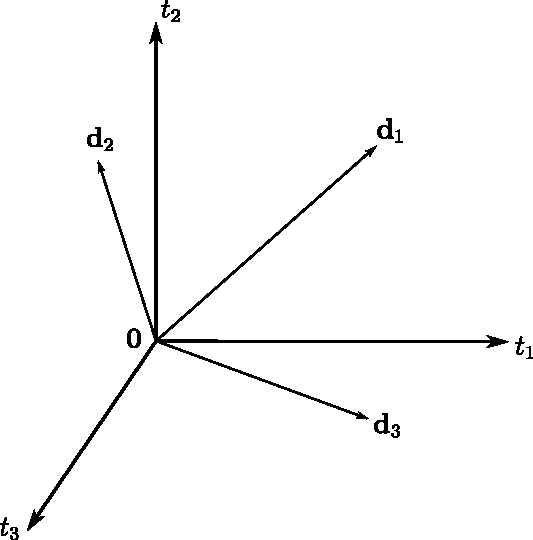
\includegraphics[width=0.5\textwidth]{document-vsm.pdf}
\caption{Documents $\mathbf d_1, \mathbf d_2, \mathbf d_3$
in a document space with dimensions $t_1, t_2, t_3$.}
\label{fig:document-vsm}
\end{figure}


There are the following term weighting schemes \cite{manning2008introduction}:

\begin{itemize}
\itemsep1pt\parskip0pt\parsep0pt
  \item binary: 1 if a term is present, 0 otherwise;
  \item term frequency (TF): number of occurrences of the term in a document;
  \item document frequency (DF): number of documents containing the terml
  \item TF-IDF: combination of TF and inverse DF.
\end{itemize}


\textbf{Term Frequency (TF)} weights terms by local frequency in the document.
That is, the term is weighed by how many times it occurs in the document.
Sometimes a term is used too often in a document, and we want to
reduce its influence, and this is typically done by applying some
sublinear transformation to TF, for instance, a square root or a logarithms.

\textbf{Document Frequency (DF)} weights terms by their global frequency
in the collection, which is the number of documents that contain the token.
But more often we are interested in domain specific words than in neutral words,
and these domain specific words tent to occur less frequently and they usually
have more discriminative power: that is, they are better in telling one document apart from another. So we use \textbf{Inverse Document Frequency (IDF)} to give more
weight to rare words rather than to frequent words.

A good weighting system gives the best performance when it assigns
more weights to terms with high TF, but low DF \cite{salton1988term}.
This can be achieved by combining both TF and IDF
schemes. Usually a sublinear TF is used to avoid the dominating effect of
words that occur too frequently. As the result, terms appearing
too rarely or too frequently are ranked low.
The TF and IDF are combined together in \textbf{TF-IDF} weighting scheme:
$$\text{tf-idf}(t, \mathbf d) = (1 + \log \text{tf}(t, \mathbf d)) \cdot \log \cfrac{n}{\text{df}(t)} \, ,$$
where $\text{tf}(t, \mathbf d)$ is term frequency of term $t$ in document
$\mathbf d$ and $\text{df}(t)$ is the document frequency of term $t$ in
the document collection.


\subsection{Similarity Measures and Distances} \label{sec:similarity-distance}

Once the documents are represented in some vector space, we need to
define how to compare these documents to each other. There are two
ways of doing this: using a similarity function that computes how similar
two objects are (the higher values, the more similar the objects),
or using a distance function, sometimes called ``dissimilarity function'',
which is the opposite of similarity (the higher the values, the less similar
the objects).

We consider Euclidean distance, inner product, cosine similarity and
Jaccard coefficient.


\subsubsection{Euclidean Distance} \ \\

The Euclidean distance function (also called length or $L_2$ norm) 
is the most commonly used distance function in vector spaces. 
Euclidean distance corresponds to the geometric distance between two data 
points in the vector space. Let $\mathbf x, \mathbf y \in \mathbb R^n$, then 
the Euclidean distance between $\mathbf x$ and $\mathbf y$ is defined 
as $\| \mathbf x - \mathbf y \| = \sqrt{\sum_{i = 1}^n (x_i - y_i)^2}$.


This distance is useful for low-dimensional data, but it does not always work
well in high dimensions, especially with sparse vector such as
document vectors \cite{ertoz2003finding}, and this effect is often called 
``Curse of Dimensionality'' \cite{beyer1999nearest}.


\subsubsection{Inner product} \ \\

The inner product between two vectors can be used as a similarity function:
the more similar two vectors are, the larger is their inner product.
Geometrically the inner product between two vectors $\mathbf x$ and $\mathbf y$
is defined as
$\mathbf x^T \mathbf y = \|\mathbf x \| \, \| \mathbf y \| \, \cos \theta$
where $\theta$ is the angle between vectors $\mathbf x$ and $\mathbf y$.
In Linear Algebra, however, the inner product
is defined as a sum of element-wise products of two vectors:
given two vectors $\mathbf x$ and $\mathbf y$, the inner product is
$\mathbf x^T \mathbf y = \sum_{i = 1}^n x_i \, y_i$ where $x_i$ and $y_i$
are $i$th elements of $\mathbf x$ and $\mathbf y$, respectively.
The geometric and algebraic definitions are equivalent \cite{huges2013calculus}.



\subsubsection{Cosine Similarity} \label{sec:cosine} \ \\


% However the magnitude of each individual vector still matters. If one
% document vector is particularly long compared to other vectors and it is not
% orthogonal to them (i.e. $\cos \theta \ne 0$), then it is likely to be
% one of the most similar vectors to others -- only because of its length.


Inner product is sensitive to the length of vectors, and thus
it may make sense to consider only the angle between them:
the angle does not depend on the magnitude, but it is still
a very good indicator of vectors being similar or not.

The angle between two vectors can be calculated from the geometric
definition of inner product:
$\mathbf x^T \mathbf y = \|\mathbf x \| \, \| \mathbf y \| \, \cos \theta$.
By rearranging the terms we get
$\cos \theta = \mathbf x^T \mathbf y \, / \, (\|\mathbf x \| \, \| \mathbf y \|)$.

We do not need the angle itself and can use the cosine directly
\cite{manning2008introduction}.
Thus can define \emph{cosine similarity} between two documents $\mathbf d_1$ and
$\mathbf d_2$ as
$$\text{cosine}(\mathbf d_1, \mathbf d_2) = \cfrac{\mathbf d_1^T \mathbf d_2}{\|\mathbf d_1 \| \, \| \mathbf d_2 \|} \ .$$
If the documents have unit lengths, then cosine similarity is the same as
dot product: $\text{cosine}(\mathbf d_1, \mathbf d_2) = \mathbf d_1^T \mathbf d_2$.

The cosine similarity can be converted to a distance function.
The maximal possible cosine is 1 for two identical documents.
Therefore we can define \emph{cosine distance} between two vectors
$\mathbf d_1$ and $\mathbf d_2$ as
$d_c(\mathbf d_1, \mathbf d_2) = 1 - \text{cosine}(\mathbf d_1, \mathbf d_2)$.
The cosine distance is not a proper metric \cite{korenius2007principal},
but it is nonetheless useful.

The cosine distance and the Euclidean distance are connected \cite{korenius2007principal}.
For two unit-normalized vectors $\mathbf d_1$ and $\mathbf d_2$ the Euclidean distance
between them is $\| \mathbf d_1 - \mathbf d_2 \|^2 = 2 - 2 \, \mathbf d_1^T \mathbf d_2 =2 \, d_c(\mathbf d_1, \mathbf d_2)$. Thus we can use Euclidean distance on
unit-normalized vectors and interpret it as cosine distance.


\subsubsection{Jaccard Coefficient} \ \\

Finally, the Jaccard Coefficient is a function that compares how similar
two sets are. Given two sets $A$ and $B$, it is computed as
$J(A, B) = \frac{|A \cap B|}{|A \cup B|}$.
It is also applicable to document vectors with binary weights, and it can
be defined as $J(\mathbf d_1, \mathbf d_2) =
\frac{\mathbf d_1^T \mathbf d_2}{\| \mathbf d_1^T \|^2 + \| \mathbf d_2^T \|^2 - \mathbf d_1^T \mathbf d_2}$ \cite{manning2008introduction}.



\subsection{Document Clustering Techniques} \label{sec:doc-clustering}

Cluster analysis is a set of techniques for organizing collection
of items into coherent groups. In Text Mining clustering is often
used for finding topics in a collection of document \cite{aggarwal2012survey}.
In Information Retrieval clustering is used to assist the users and group
retrieved results into clusters \cite{cutting1992scatter}.

There are several types of clustering algorithms:
hierarchical (agglomerative and divisive), partitioning,
density-based, and others.


\subsubsection{Agglomerative clustering} \label{sec:clustering-heierarchical} \ \\

The general idea of agglomerative clustering algorithms is to start with
each document being its own cluster and iteratively merge clusters based
on best pair-wise cluster similarity.

Thus, a typical agglomerative clustering algorithms consists of the following steps:

\begin{enumerate}
\itemsep1pt\parskip0pt\parsep0pt
  \item Let each document be a cluster on its own;
  \item Compute similarity between all pairs of clusters an store the
      results in a similarity matrix;
  \item Merge two most similar clusters;
  \item Update the similarity matrix;
  \item Repeat until everything belongs to the same cluster.
\end{enumerate}

These algorithms differ only in the way they calculate similarity between
clusters. It can be \textbf{Single Linkage}, when the clusters are merged based
on the closest pair; \textbf{Complete Linkage}, when the clusters are merged
based on the worst-case similarity -- the similarity between the most
distant objects on the clusters; \textbf{Group-Average Linkage}, based
on the average pair-wise similarity between all objects in the clusters;
and \textbf{Ward's Method} when the clusters to merge are chosen to
minimize the within-cluster error between each object and its centroid
is minimized \cite{oikonomakou2005review}.

Among these algorithms only Single Linkage is computationally feasible
for large data sets, but it doesn't give good results compared to other
agglomerative clustering algorithms. Additionally, these algorithms
are not always good for document clustering because they tend to
make mistakes at early iterations that are impossible to correct
afterwards \cite{steinbach2000comparison}.



\subsubsection{$K$-Means} \label{sec:kmeans} \ \\

Unlike agglomerative clustering algorithms, K-Means is an iterative
algorithm, which means that it can correct the mistakes made
at earlier iterations. Lloyd's algorithm is the most popular way
of implementing K-Means \cite{xu2005survey}: given a desired number of clusters $K$,
it iteratively improves the Euclidean distance between each data
point and the centroid, closest to it.


Let $\mathcal D = \{  \mathbf d_1, \mathbf d_2, \ ... \ , \mathbf d_n \}$
be the document collection, where documents $\mathbf d_i$ are represented
is a document vector space $\mathbb R^m$ and $K$ is the desired
number of clusters. Then we define $k$ cluster centroids $\boldsymbol \mu_j$ that are
also in the same document vector space $\mathbb R^m$.
Additionally for each document $\mathbf d_i$ we maintain the assignment
variable $c_i \in \{ 1, 2, \ ... \ , k \}$, which specifies to what
cluster centroid $\boldsymbol \mu_1, \boldsymbol \mu_2, \ ... \ , \boldsymbol \mu_k$
the document $\mathbf d_i$ belongs.


The algorithms consists of three steps: (1) seed selection step,
where each $\boldsymbol \mu_j$ is randomly assigned some value,
(2) cluster assignment step, where we iterate over all document vectors
$\mathbf d_i$ and find its closest centroid, and (3)  move centroids step,
where the centroids are re-calculated. Steps (2) and (3) are repeated
until the algorithm converges. The pseudocode for $K$-Means is presented
in the listing~\ref{algo:k-means}.

\begin{algorithm}
\caption{Lloyd's algorithm for $K$-Means}
\label{algo:k-means}

\begin{algorithmic}[0]
  \Statex
  \Function{K-Means}{no. clusters $k$, documents $\mathcal D$}
    \For{$j \leftarrow 1 \ .. \ k$} \Comment{random seed selection}
      \Let{$\boldsymbol \mu_j$}{random $\mathbf d \in \mathcal D$}
    \EndFor

    \While{not converged}
      \For{each $\mathbf d_i \in \mathcal D$} \Comment{cluster assignment step}
        \Let{$c_i$}{$\operatorname{arg\, min}_j \| \mathbf d_i - \boldsymbol \mu_j \|^2$}
      \EndFor

      \For{$j \leftarrow 1 \ .. \ k$} \Comment{move centroids step}
        \Let{$\mathcal C_j$}{$\{\, \mathbf d_i \text{ s.t. } c_i = j \, \}$}
        \Let{$\boldsymbol \mu_j$}
            {$\cfrac{1}{| \mathcal C_j |} \sum_{\mathbf d_i \in \mathcal C_j} \mathbf d_i$}
      \EndFor
    \EndWhile

    \State \Return{$(c_1, c_2, \ ... \ , c_n)$}
  \EndFunction
\end{algorithmic}
\end{algorithm}

Usually, $K$-Means shows very good results for document clustering, and in
several studies it (or its variations) shows the best performance
\cite{steinbach2000comparison} \cite{hall2012evaluating} .

However for large document collections Lloyd's classical $K$-Means takes a lot
of time to converge. The problem is caused by the fact that it goes through
the entire collection many times. Mini-Batch $K$-Means \cite{sculley2010web}
uses Mini-Batch Gradient Descent method, which is a different optimization technique
that converges faster.

$K$-Means uses Euclidean distance, which does not always behave
well in high-dimensional sparse vector spaces like document vector
spaces. However, as discussed in section~\ref{sec:similarity-distance}, if
document vectors are normalized, the Euclidean distance and cosine distance
are related, and therefore Euclidean $K$-means is the same as
``Cosine Distance'' $K$-Means.

% $K$-Means is the most popular clustering algorithms and there are
% many extensions. For example, Bisecting K-Means
% \cite{steinbach2000comparison} is a combination
% of partitioning and hierarchical (divisive) algorithms. It's a
% variant of $K$-Means that gradually splits the document space in halves
% until the desired number of clusters is obtained. Bisecting $K$-Means can
% achieve good performance while giving the user additional insight into
% the clustering process. Additionally, in the results it produces
% clusters of comparable sizes.

% The algorithm is simple: (1) start with a single cluster;
% (2) choose a cluster to split (for example, the largest one);
% (3) apply traditional $K$-Means to this cluster with $K=2$ to split it;
% (4) repeat until have desired number of clusters.

In cases when there are many documents, the centroids tend to contain a lot of words, 
which leads to a significant slowdown. To solve this problem, some terms of the 
centroid can be truncated. There are several possible ways of truncating the 
terms: for example, we can keep only the top $c$ terms, or remove the least 
frequent words such that at least 90\% (or 95\%) of the original vector norm is
retained \cite{schutze1997projections}.


\subsubsection{DBSCAN} \label{sec:dbscan} \ \\

DBSCAN is a density-based clustering algorithm that can discover
clusters of complex shapes based on the density of data points \cite{ester1996density}.

The \emph{density} associated with a data point is obtained by
counting the number of points in a region of radius $\varepsilon$
around the point, where $\varepsilon$  is defined by the user.
If a point has a density of at least some user defined
threshold \verb|MinPts|, then it is considered a \emph{core point}.
The clusters are formed around these core points, and if two core points
are within the radius $\varepsilon$, then they belong to the same cluster.
If a point is not a core point itself, but it belong to the neighborhood of some
core point, then it is a \emph{border point}. But if a point is not a core point
and it is not in the neighborhood of any other core point, then it does not
belong to any cluster and it is considered \emph{noise}.

DBSCAN works as follows: it selects an arbitrary data point $p$, and then
finds all other points in $\varepsilon$-neighborhood of $p$. If
there are more than  \verb|MinPts| points around $p$, then it is a core point,
and it is considered a cluster. Then the process is repeated for all points in
the neighborhood, and they all are assigned to the same cluster, as $p$.
If $p$ is not a core point, but it has a core point in its neighborhood, then
it's a border point and it is assigned to the same cluster and the core point.
But if it is a noise point, then it is marked as noise or discarded
(see listing~\ref{algo:dbscan}).


\begin{algorithm}
\caption{DBSCAN}
\label{algo:dbscan}

\begin{algorithmic}[0]
  \Statex
  \Function{DBSCAN}{database $\mathcal D$, radius $\varepsilon$, MinPts}
    \Let{$\text{result}$}{$\varnothing$}

    \ForAll{$p \in \mathcal D$}
      \If{$p$ is visited}
        \State{\textbf{continue}}
      \EndIf
      \State{mark $p$ as visited}
      \Let{$\mathcal N$}{\textsc{Region-Query}($p, \varepsilon$)}
          \Comment{$\mathcal N$ is the neighborhood of $p$}
      \If{$\mathcal N < \text{MinPts}$}
        \State{mark $p$ as \texttt{NOISE}}
      \Else
        \Let{$\mathcal C$}
            {\textsc{Expand-Cluster}$(p, \mathcal N, \varepsilon, \text{MinPts})$}
        \Let{result}{result $\cup \ \{ \mathcal C \}$}
      \EndIf
    \EndFor
    \State \Return{result}
  \EndFunction
\end{algorithmic}


\begin{algorithmic}[0]
  \Statex
  \Function{Expand-Cluster}{point $p$, neighborhood $\mathcal N$, radius $\varepsilon$, MinPts}
     \Let{$\mathcal C$}{$\{ p \}$}
     \ForAll{$x \in \mathcal N$}
        \If{$x$ is visited}
          \State{\textbf{continue}}
        \EndIf

        \State{mark $x$ as visited}
        \Let{$\mathcal N_x$}{\textsc{Region-Query}$(x, \varepsilon)$}
            \Comment{$\mathcal N_x$ is the neighborhood of $x$}
        \If{$| \mathcal N_x | \geqslant \text{MinPts}$}
          \Let{$\mathcal N$}{$\mathcal N \cup \mathcal N_x$}
        \EndIf

        \Let{$\mathcal C$}{$\mathcal C \cup \{ x \}$}
     \EndFor

     \State \Return{$\mathcal C$}
  \EndFunction
\end{algorithmic}

\begin{algorithmic}[0]
  \Statex
  \Function{Region-Query}{point $p$, radius $\varepsilon$}
     \State \Return{$\{ x \ : \ \| x - p \| \leqslant \varepsilon \}$} \Comment{all points within distance $\varepsilon$ from $p$}
  \EndFunction
\end{algorithmic}

\end{algorithm}

The details of implementation of \textsc{Region-Query} are not specified,
and it can be implemented differently. For example, it can use
Inverse Index to make the similarity search faster
\cite{manning2008introduction} \cite{ertoz2003finding}.


The DBSCAN algorithm uses the Euclidean distance, but can be adapted to
use any other distance or similarity function. For example, to modify the
algorithm to use the cosine similarity (or any other similarity function)
the \textsc{Region-Query} has to be modified to return
$\{ x \ : \ \text{similarity}(x, p) \geqslant \varepsilon \}$.

Shared Nearest Neighbors Similarity (SNN Similarity) \cite{ertoz2003finding}
is a special similarity function that is particularity useful for
high-dimensional spaces, it works well with DBSCAN, and it is
applicable to document clustering and topic discovery \cite{ertoz2004finding}.

SNN Similarity is specified in terms of the $K$ nearest neighbors.
Let $\text{NN}_{K, \, \text{sim}}(p)$ be a function that returns
top $K$ closest points of $p$ according to some similarity function
\texttt{sim}. Then the SNN similarity function is  defined as
$$\text{snn}(p, q) = \big| \text{NN}_{K, \, \text{sim}}(p) \cup \text{NN}_{K, \, \text{sim}}(q) \big|.$$


The extension of DBSCAN that uses the SNN Similarity is called
SSN Clustering algorithm. The user needs to specify the SSN similarity
function by setting parameter $K$ and choosing the base similarity
function $\text{\texttt{sim}}(\cdot, \cdot)$ (typically Cosine, Jaccard
or Euclidean). The algorithm itself has the same
parameters as DBSCAN: radius $\varepsilon$ (such that $\varepsilon < K$)
and the core points density threshold \verb|MinPts|. The
$\textsc{Region-Query}$ function is modified to return
$\{ q \ : \ \text{snn}(p, q) \geqslant \varepsilon \}$. For pseudocode,
see the listing~\ref{algo:snn-clustering}.

\begin{algorithm} \caption{SNN Clustering Algorithm} \label{algo:snn-clustering}

\begin{algorithmic}[0]
  \Statex
  \Function{SNN-Cluster}{database $\mathcal D$, $K$, similarity function \texttt{sim}, radius $\varepsilon$, MinPts}
    \ForAll{$p \in \mathcal D$} \Comment{Pre-compute the $K$NN lists}
      \Let{$\text{NN}[p]$}{$\text{NN}_{K, \, \text{sim}}(p)$}
    \EndFor

    \ForAll{$(p, q) \in (\mathcal D \times \mathcal D)$} \Comment{Pre-compute the SNN similarity matrix}
      \Let{$A[p, q]$}{$\big| \, \text{NN}[p] \ \cup \ \text{NN}[q] \, \big|$}
    \EndFor

    \State \Return{\textsc{DBSCAN}$(A, \varepsilon, \text{MinPts})$}
  \EndFunction
\end{algorithmic}

\end{algorithm}


The algorithm's running time complexity is $O(n^2)$ time, where $n = |\mathcal D|$,
but it can be sped up by using the Inverted Index \cite{ertoz2003finding}.


\subsection{Latent Semantic Analysis} \label{sec:lsa}

In section~\ref{sec:clusters-namespaces} we have discussed the
lexical variability and ambiguity problems in natural language: synonymy
and polysemy. We can treat these problems as ``statistical noise'' and
apply dimensionality reduction techniques to find the optimal dimensionality
for the data and thus reduce the amount of noise there.
This technique is called Latent Semantic Analysis (LSA) \cite{landauer1998introduction}
or Latent Semantic Indexing \cite{deerwester1990indexing}, and
it is often used for document clustering \cite{aggarwal2012survey} \cite{osinski2004lingo}.

There are three major steps in Latent Semantic Analysis  \cite{evangelopoulos2012latent}:
(1) preprocess documents;
(2) construct a term-document matrix $D$ using the Vector Space Model;
(3) de-noise $D$ by reducing its dimensionality with Singular Value Decomposition (SVD).

The first two steps are the same as for traditional Vector Space Models
and in the result we obtain a term-document matrix $D$.
If $D$ has rank $r$, then the SVD of $D$ is $D = U  \Sigma V^T$, where
$U$ is an $m \times r$ orthogonal matrix;
$\Sigma$ is a diagonal $r \times r$ matrix with singular values ordered by their magnitude;
and $V$ is an $n \times r$ orthogonal matrix.

The dimensionality reduction is done by finding the best $k$-rank approximation
of $D$, which is obtained by keeping only the first $k$ singular values of $\Sigma$
and setting the rest to 0.
Typically, not only $\Sigma$ is truncated, but also $U$ and $V$,
and therefore, the $k$-rank approximation of $D$ using SVD is written as
$D \approx D_k = U_k \Sigma_k V_k^T$ where $U_k$ is an $m \times k$
matrix with first $k$ columns of $U$, $\Sigma_k$ is an $k \times k$
diagonal matrix with singular values, and $V_k$ is an $n \times k$
matrix with first $k$ columns of $V$.  This decomposition
is called \emph{rank-reduced} SVD and when applied to text data
it reveals the ``true'' latent semantic space. The parameter $k$ corresponds
to the number of ``latent concepts'' in the data. The idea
of LSA is very nicely illustrated by examples  in
\cite{deerwester1990indexing} and \cite{landauer1998introduction}.

LSA can be used for clustering as well, and this is usually done
by first transforming the document space to the LSA space
and then doing applying transitional cluster analysis techniques
there \cite{schutze1997projections}.
Once $D$ is decomposed as $D \approx U_k \Sigma_k V_k^T$
it is enough to keep only the low dimensional representation $\hat D = V_k \Sigma_k$:
the calculation of inner product between two documents $i$ and $j$ in
the reduced semantic  space corresponds to computing the inner product
between $i$th and $j$th rows of $\hat D$ \cite{deerwester1990indexing}. Since the
Euclidean distance is defined in terms of inner product, it can also be used
directly on the rows of $\hat D$.

Therefore, a generic LSA-based clustering algorithm consists of the following steps:

\begin{enumerate}
\itemsep1pt\parskip0pt\parsep0pt
  \item Build a term-document matrix $D$ from the document collection;
  \item Select number of latent concepts $k$ and apply rank-reduced SVD on $D$
      to get $\hat D= V_k \Sigma_k$;
  \item Apply the cluster algorithm on the rows of $V_k \Sigma_k$.
\end{enumerate}


LSA has some drawbacks. Because SVD looks for an orthogonal basis for the new
reduced document space, there could be negative values that are harder
to interpret, and what is more, the cosine similarity can become negative as well.
However, it does not significantly affect the cosine distance: it still
will always give non-negative results.

Apart from SVD there are many other different matrix decomposition
techniques that can be applied for document clustering and for discovering
the latent structure of the term-document matrix \cite{osinski2006improving},
and one of them in Non-Negative Matrix Factorization (NMF) \cite{lee1999nnmf}.
Using NMF solves the problem of negative coefficients:
when it is applied to non-negative data such as term-document matrices,
NMF produces non-negative rank-reduced approximations.

The main conceptual difference between SVD and NMF is that SVD looks for
orthogonal directions to represent document space, while NMF does not
require orthogonality \cite{xu2003document} (see fig.~\ref{fig:nmf-svd}).


\begin{figure}[h]
\centering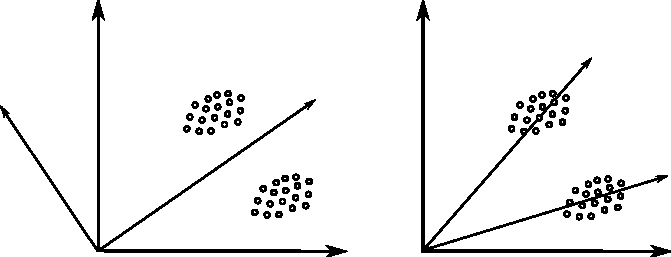
\includegraphics[width=0.8\textwidth]{nmf-svd.pdf}
\caption{Directions found by  SVD (on the left) vs directions by NMF (on the right)}
\label{fig:nmf-svd}
\end{figure}


The NMF of an $m \times n$ term-document matrix $D$ is $D \approx D_k = U  V^T$
where $U$ is an $m \times k$ matrix, $V$ is an $n \times k$ matrix and
$k$ is the number of semantic concepts in $D$.
Non-negativity of elements in $D_k$ is very good for interpretability: it
ensures that documents can be seen as a non-negative combination of
the key concepts.

Additionally, NMF is useful for clustering: the results of NMF can
be directly interpreted as cluster assignment and there is no need
to use separate clustering algorithms \cite{xu2003document}. When $D$ is a
term-document matrix and $D \approx U V^T$, then elements $(V)_{ij}$
represent the degree to which document $i$ belongs to cluster $j$.

The document clustering using NMF consists of the following steps \cite{xu2003document}:

\begin{enumerate}
  \item Construct the term-document matrix $D$ and perform NMF on $D$ to get $U$ and $V$;
  \item Normalize rows $\mathbf v_i$ of $V$ by using the rule $\mathbf v_i \leftarrow \mathbf v_i \, \| \mathbf u_i \|$;
  \item Assign document $\mathbf d_i$ to cluster $x$ if $x = \operatorname{arg \, max}_j (V)_{ij}$.
\end{enumerate}

If the desired number of clusters $K$ is larger than the rank $k$ of the
reduced matrix $D_k$, the clustering can be performed directly on the rows
of $V$, for example, by using $K$-Means.

% The computational complexity on NMF is $O(kn)$
